\chapter{Analysis of security tools for the pipeline}
\label{chap:Tools}
\section{Introduction}
The following chapter presents tools that can be utilized as the security tools implemented in the \gls{pipeline} presented in Chapter \ref{Pipeline security}. Additionally, the group will explain the reasoning behind selecting each of the different tools and look at the advantages and disadvantages of each tool. 

\section{OWASP ZAP}
\acrshort{owasp} \acrlong{zap} (\acrshort{owasp} \acrshort{zap})\footnote{Available at \url{https://www.zaproxy.org/}} is an open-source web application security scanner \cite{owaspZAP}. It is free and maintained by volunteers worldwide under the \acrlong{owasp}. \acrshort{zap} is a \acrshort{dast} tool and is designed to test web application security. The tool offers functionality for many people - from developers to experienced testers. It is available in versions that are compatible with major operating systems, as well as Docker\footnote{Available at: https://www.docker.com/}, which means that users are not limited to a specific operating system when using the tool.

\subsection{OWASP ZAP: advantages and disadvantages}
The following advantages and disadvantages combine the personal experiences and information found during research.\cite{prosconsZAP}
\begin{table}[H]
    \begin{threeparttable}
        \begin{tabular}{|>{\raggedright\arraybackslash}p{6cm}|>{\raggedright\arraybackslash}p{6cm}|}
            \hline
            \textbf{Advantages} & \textbf{Disadvantages} \\
            \hline
            \begin{itemize}
                \item [-]\textbf{Open source:} It is open source, which allows users to access it without paying for it. 
                \item [-]\textbf{Configuration:}Easy to configure with \acrshort{aws}
                \item [-]\textbf{Many available:}There are multiple application security testing approaches available that can help discover potential vulnerabilities
            \end{itemize}
            &
            \begin{itemize}
                \item [-] \textbf{Documentation:}The documentation could be improved and is, for some, difficult to understand
                \item [-]\textbf{Compare:} Compared to other tools, the automated scanning features are restricted
            \end{itemize}
            \\
            \hline
        \end{tabular}
            \caption{Advantages and disadvantages of OWASP ZAP}
    \end{threeparttable}
\end{table}


\section{GitHub security Tools}
Below are the GitHub tools that can be utilized to conduct a wide range of application security testing on the code sent through the pipeline. 

\subsection{Dependabot}
Dependabot is an in-built GitHub tool that helps developers keep their project dependencies up-to-date and is an example of an \acrshort{sca} tool that can be used in the implementation phase \cite{GithubDependabot1}.
\\~\\
Dependencies can be updated over time as new versions are released. Therefore, developers must keep the dependencies current to ensure the project stays secure. However, keeping track of all updates that come and manually running these updates can be rather time-consuming and error-prone. Dependabot automates checking for new versions of the dependencies used in the code and then creates a pull request to update them. The user can then review the updates and see if it is necessary to make any changes. 
Dependabot can also automatically resolve any conflict that may arise when updating dependencies and can open up separate pull requests for separate dependency updates. 
\\~\\
Dependabot uses the \say{GitHub Advisory Database} to check for vulnerable data. This database covers a lot of public vulnerabilities, and it uses multiple sources, like \acrlong{cve}, explained in \ref{Common Vulnerabilities and Exposures}, \acrlong{nvd}, and several others. \cite{GithubDependabot2}


\subsubsection{Dependabot: advantages and disadvantages}
These advantages and disadvantages combine the personal experiences and information found during research. \cite{prosconsdependabot} 

\begin{table}[H]
\centering
\begin{tabular}{|>{\raggedright\arraybackslash}p{6cm}|>{\raggedright\arraybackslash}p{6cm}|}
\hline
\textbf{Advantages} & \textbf{Disadvantages} \\
\hline
\begin{itemize}
\item [-]\textbf{Automated:} It Automates dependency updates, saving time and reducing manual errors 
\item [-] \textbf{Support:} It supports a wide range of languages and package managers 
\item [-]\textbf{Change-logs:} It Provides detailed change-logs and release notes 
\end{itemize}
&
\begin{itemize}
\item [-] \textbf{Merge conflict:} Can create merge conflicts with other changes 
\item [-] \textbf{False-positives:} The automatic scan of Dependabot may generate many false positives, which can be time-consuming to rectify. Getting false positives requires users to manually review each issue to determine whether a change is necessary. 

\end{itemize}
\\
\hline
\end{tabular}
\caption{Advantages and disadvantages of Dependabot}
\label{tab:dependabot}
\end{table}

\subsection{CodeQL}
GitHub has an in-built code scanning tool called CodeQL that allows the users to analyze the code in the GitHub repository to find vulnerabilities and errors in the code \cite{CodeQL1}. This tool can be used as the \acrshort{sast} tool in the \gls{pipeline}. CodeQL is also a recommended tool according to Microsoft's best practice for secure \acrshort{sdlc} that argues using approved tools \cite{microsoftSDLCpractices}. The results of these analyzes are shown as code-scanning alerts in GitHub. This feature helps identify existing issues and prevents new ones from being introduced. 
\\~\\
CodeQL can be scheduled so that it runs on chosen days or occurrences of events. For example, rather than scanning each branch individually, it is possible to set up a trigger that will initiate the code scan only when the code is pushed to the main branch or when a pull request is made. Limiting the triggers helps to reduce the amount of time and resources required to perform the scans. Also, it minimizes the risk of vulnerabilities or errors being introduced into the production environment.
\\~\\
Any issues found during the scanning process are displayed as alerts within the repository. This means that developers can divide the different issues easily between team members. Once a user fixes the code that triggered the alert, it is automatically closed. Additionally, users can monitor the results of code scanning across their repositories or organization using web-hooks and the code scanning API. 
\cite{GithubCodeScanning}

\begin{comment}
    CodeQL and Dependabot have together detected 101 vulnerabilities. This is the exact number of vulnerabilities "...intentionally planted in the application..." \cite{owaspJuiceShop}.
\end{comment}

\subsubsection{CodeQL: advantages and disadvantages}
\begin{table}[H]
\centering
\begin{tabular}{|>{\raggedright\arraybackslash}p{6cm}|>{\raggedright\arraybackslash}p{6cm}|}
\hline
\textbf{Advantages} & \textbf{Disadvantages} \\
\hline
\begin{itemize}
\item [-] \textbf{Create triggers:} Teams can decide when to trigger the scanning. This is usually when an event occurs, such as pull requests
\item [-]\textbf{Suitable for projects:} The scan can be configured so that it tailors the different needs
\item [-] \textbf{Auto-build:} When code scanning runs, it automatically uploads the vulnerabilities it found to the repository's security tab
\end{itemize}
&
   \begin{itemize}
\item [-]\textbf{Precision:} The precision can depend on the code. If the code requires a specific type of customization, then the precision of the default setup for CodeQL will not necessarily be that suitable. 
\item [-] \textbf{Language support:}Only supports a smaller set of languages 
\end{itemize}
\\
\hline
\end{tabular}
\caption{Advantages and disadvantages of CodeQL}
\label{tab: CodeQL}
\end{table}


\subsection{Secret Scanner}
To prevent fraudulent use of accidentally committed secrets, GitHub scans repositories and archived repositories for known secrets \cite{GithubSecretScanning}. Secret Scanner is provided in two forms:  

\begin{itemize}
    \item [-] \textbf{Secret Scanning alerts for partners}\\
    When a repository is made public, or changes have been pushed to a public repository on GitHub, the code is automatically scanned for any secrets that match the patterns of GitHub's partners. The Secret Scanner also scans for credentials in the public package registry, like the npm registry\footnote{Available at: https://www.npmjs.com/}. GitHub notifies the associated service provider when the scanner detects a secret. The provider will validate the secret and decide what the course of action will be, for example, revoking the secret or creating an issue. The specific action will depend on the level of risk involved. 
    
    \item [-] \textbf{Secret Scanning alerts for users}\\
    Secret Scanning alerts for users are free for all public repositories. By enabling secret scanning for a repository, the scanner will look for patterns in the code that could match secrets by different service providers. Once the scan is complete, GitHub sends an email alert to the enterprise and the owners of the organizations. However, if a secret has been compromised, GitHub generates an alert for secret scanning. 
    
\end{itemize}

\subsubsection{Secret Scanner: advantages and disadvantages}
\begin{table}[H]
\centering
\begin{tabular}{|>{\raggedright\arraybackslash}p{6cm}|>{\raggedright\arraybackslash}p{6cm}|}
\hline
\textbf{Advantages} & \textbf{Disadvantages} \\
\hline
\begin{itemize}
\item [-] \textbf{Free:} GitHub has given public access to this feature 
\item [-]\textbf{Convenience:} As projects become more complex and it becomes harder to keep track of all the secrets stored in the repository, Secret Scanner will help detect these faster 
\item [-] \textbf{Secure:} Secrets can be easily missed when writing large amounts of code. Enabling Secret Scanning can potentially increase the security 
\end{itemize}
&
   \begin{itemize}
\item [-] \textbf{False positives:} Secret Scanning cannot always determine if the secret is legitimate or not, which occasionally can occur in false positives
\item [-] \textbf{Limited Coverage:} It can be limited and does not always detect all secrets created manually, such as personal passwords. 
    \end{itemize}
    \\
    \hline
    \end{tabular}
    \caption{Advantages and disadvantages of GitHub´s Secret Scanner}\cite{Secret_Scanner_pros_cons}
    \label{tab: Secret_Scanner}
    \end{table}
    
\newpage
\subsection{Branch Protection}
\label{branchprotection}
Branch protection is a feature of GitHub that enforces different rules and requirements for specific branches in the repository \cite{ProtectedBranches}. The purpose of branch protection is to maintain the code's security, which is done by ensuring that all changes done to the branch have gone through the proper steps before being merged into the main branch. Figure \ref{fig: Pipeline with implemented branch protection rules} demonstrates that branch protection is enabled before code is pushed to GitHub in order for the source code to enter a secure repository. Below are the different branch protection features that can be enabled in GitHub. 

\subsubsection{Require a pull request before merging}
Administrators of the repository can add rules to the repository which restrict pull requests to have a specific number of people approving the changes before merging to a protected branch. Administrators can allow code owners and users with written permissions to approve.
\\~\\
Under this type of protection, the "Four Eyes Principle" is applied. Since this type of protection requires that at least two people approve the merge, this includes the person doing the changes. This principle can be considered a controlling mechanism that improves the quality of the outcome, minimize risk errors, and prevents malicious actions by a single individual. 

\subsubsection{Require status checks before merging}
Maintaining high code quality is essential when multiple users collaborate within a shared repository. By enabling the \say{require status checks to pass before merging} feature, repository administrators can establish specific criteria that must be met before code is merged, such as requiring code approval from at least one team member.

\subsubsection{Require conversation resolution before merging}
When working together on the same repository, it is essential to have clear communication and collaboration. A way to secure this is to enable \say{require conversation resolution before merging}. Enabling this rule allows all discussions regarding, for example, issues or pull requests that need to be properly resolved before any merging happens. 

\subsubsection{Require signed commits}
Enabling require \say{signed commits} can be considered a security measure that ensures that changes in the code have not been tampered with. To be able to have secured signed commits, all commits pushed to the repository must be signed with a \acrlong{gpg} (\acrshort{gpg}) key or an \acrshort{ssh} key. 


\subsubsection{Require deployments to succeed before merging}
\say{Require deployments to succeed before merging} enables users to enforce the passing of various required checks, such as pre-merge checks or automated tests, before allowing a pull request to be merged into the main branch.

\subsubsection{Lock branch}
As the name implies, the lock branch allows users to lock a branch in a repository, preventing changes from being made to the branch. This rule can be helpful if there are situations where the branch needs to be protected from unauthorized changes or to be deleted. 

\subsubsection{Do not allow bypassing the above settings}
This feature stops users from bypassing required checks and restrictions in a repository. For example, if an administrator enables a rule that all pull requests must pass reviews and checks before merging, the feature prompts users to comply before making changes to the branch.

\subsubsection{Restrict who can push to matching branches}
This branch protection can be enabled for public repositories owned by a GitHub Free organization and organizations using GitHub Team or GitHub Enterprise Cloud. When enabled, only specific users or teams with specific permissions are allowed to push any changes to the protected branch. 
\newpage
\subsubsection{Allow force pushes}
As default, GitHub prevents force pushes on all protected branches. However, \say{force pushes} can be enabled and gives two options:
\begin{itemize}
    \item [-] Allow anyone with at least writing permission, including admins, to force a push to the branch.
    \item [-] Restrict force pushing to specific individuals or teams. 
\end{itemize}
Force pushes allow users to overwrite the branch's commit history with their local commit history. 
\subsubsection{Allow deletions}
By default, GitHub restricts a user from deleting a protected branch. However, when \say{allow deletions} is enabled on a branch, anyone with only write permissions or more to the repository can delete the specific branch. 

\subsection{Branch protection: advantages and disadvantages}
\begin{table}[H]
\centering
\begin{tabular}{|>{\raggedright\arraybackslash}p{6cm}|>{\raggedright\arraybackslash}p{6cm}|}
\hline
\textbf{Advantages} & \textbf{Disadvantages} \\
\hline
\begin{itemize}
\item [-] \textbf{Code changes:} It prevents unauthorized code changes, ensuring only authorized users can make changes to a particular branch.
\item [-]\textbf{Code quality:} It can help enforce code review and approval of code, specifying the code's quality. 
\item [-] \textbf{Collaboration:} By restricting certain actions within different branches, users can work on different aspects of the project without compromising others' work towards the same goal.  
\end{itemize}
&
   \begin{itemize}
\item [-] \textbf{Create bottlenecks:} If only a few individuals are authorized to make changes, it can create bottlenecks and delays in approving different issues. 
\item [-] \textbf{Workflow:} Branch protections can quickly ruin workflows if something always needs approval before moving on. 
    \end{itemize}
    \\
    \hline
    \end{tabular}
    \caption{Advantages and disadvantages of GitHub's Branch Protection}
    \label{tab: Branch_protection}
    \end{table}
    


\section{Amazon Web Services Tools}

The following are the \acrshort{aws} tools that can be utilized in creating and deploying a web application. A range of different tools are available, but only the selected tools listed below will be utilized in the deployment process detailed in Chapter \ref{Deployment}.

\subsection{AWS CodePipeline}
\acrshort{aws} CodePipeline is a \say{\textit{...fully managed continuous delivery service that helps you automate your release \gls{pipeline}. It allows users to build, test, and deploy code into a test production environment...}} \cite{AWSCodePipeline}.
\\~\\
CodePipeline automates the entire \gls{pipeline}, including the build, test, and deploy phases, and triggers these processes whenever changes are detected in the repository. When a developer pushes changes to the repository, CodePipeline automatically detects them and initiates the process by building them. If any tests are configured, CodePipeline also runs these tests.\cite{AWSCodePipeline1}
\begin{figure}[H]
    \centering
    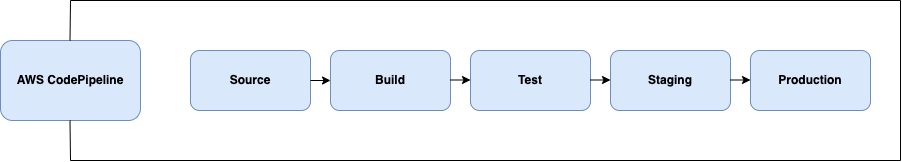
\includegraphics[scale=0.4]{Images/CodePipeline.png}
    \caption{AWS CodePipeline process}Adapted from: \cite{AWSCodePipeline2}
    \label{fig: AWS CodePipeline Process}
\end{figure}

\subsection{AWS CodeBuild }
\acrshort{aws} CodeBuild can be described as a \say{\textit{...fully managed continuous integration service that compiles source code, runs tests, and produces ready-to-deploy software packages.}} \cite{AWSCodeBuild}.
\\~\\
AWS CodeBuild downloads the source code provided to it into a build environment and then uses a \gls{buildspec}, which defines how the built project should be executed. \cite{AWSCodeBuild1}
\begin{figure}[H]
    \centering
    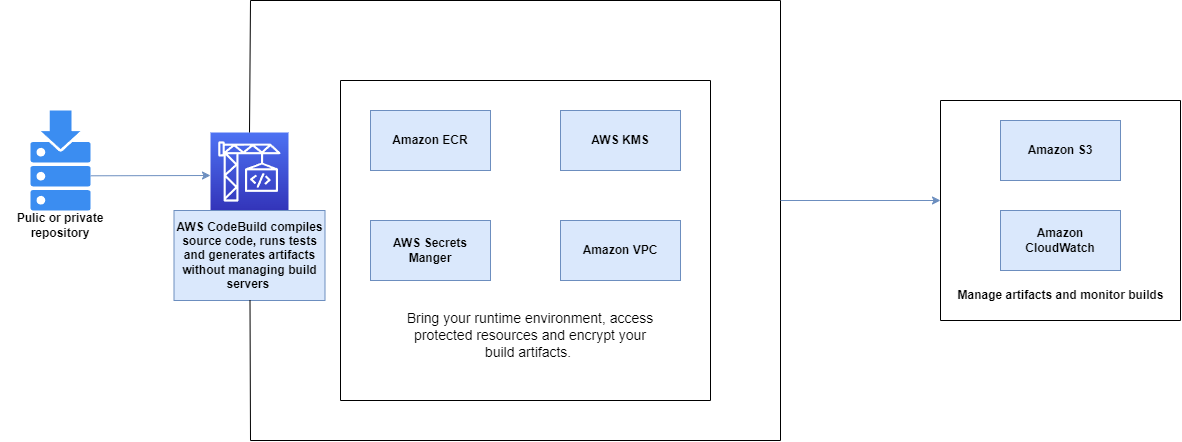
\includegraphics[scale=0.3]{Images/Codebuild.png}
    \caption{AWS CodeBuild process} Adapted from: \cite{AWSCodeBuild}
    \label{fig: AWS CodeBuild Process}
\end{figure}

\subsection{AWS CodeDeploy}
\acrshort{aws} CodeDeploy is explained as \say{\textit{...a fully managed deployment service that automates software deployments to various compute services, such as Amazon Elastic Compute Cloud (EC2), AWS Lambda and more...}} \cite{AWSCodeDeploy}.
\acrshort{aws} CodeDeploy helps developers avoid downtime during deployment. It also handles the updating phase of the applications. 
\\~\\
CodeDeploy can deploy code that runs on a server and is stored in, for example, GitHub repositories or in a \acrshort{aws} S3 Bucket. In order to use CodeDeploy, developers are not required to make any adjustments to their existing code. \cite{CodeDeploy1}

\begin{figure}[H]
    \centering
    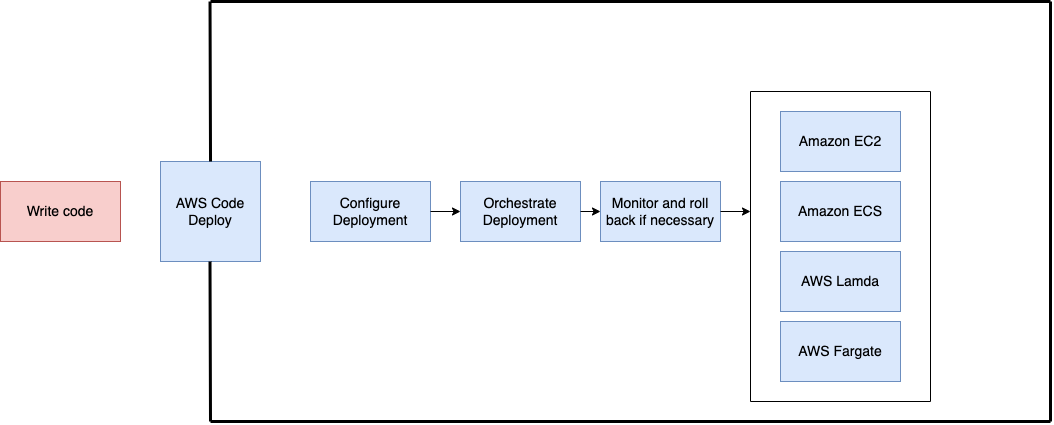
\includegraphics[scale=0.4]{Images/AWSCodeDeploy.png}
    \caption{AWS CodeDeploy process} Adapted from: \cite{CodeDeploy1}
    \label{fig: AWS CodeDeploy Process}
\end{figure}


\subsection{Amazon S3 buckets}
Amazon S3 buckets are simple, cloud-based storage resources \cite{S3Bucket}. S3 buckets are designed to provide users with scalable, durable, and highly available storage, which can be used to store different types of data. Such data can be documents, \gls{artifact}s, source code, and so on. An S3 bucket can be considered a container that stores different objects. 
\newpage
\subsection{Amazon EC2}
\acrlong{ec2} (\acrshort{ec2}) offers a \gls{compute platform}, with virtual computing environments, also known as instances \cite{awsec2}. \acrshort{ec2} offers various instance types to meet computing needs. The instance type determines the instances' CPU, memory, storage, and networking capacity. The instances are launched from \acrlong{amis} (\acrshort{amis}). \acrshort{amis} are templates that contain the necessary software configurations and operating system to run the server \cite{amis}.